\documentclass[a4paper]{article}

\usepackage[a4paper,margin=2cm]{geometry}
\usepackage{amsmath}
\usepackage{graphicx}
\usepackage[table]{xcolor}
\usepackage{tikz}
\usepackage{minted}
\usepackage[clock]{ifsym}
\usepackage{subcaption} % subfigures
\usepackage{hyperref} % links in table of contents
\usepackage[strings]{underscore}

\usetikzlibrary{calc,positioning,shapes,arrows.meta,decorations.pathreplacing}
\graphicspath{ {./graphics/} }

\hypersetup{
	colorlinks,
	citecolor=black,
	filecolor=black,
	linkcolor=black,
	urlcolor=black
}
\numberwithin{figure}{section}
\numberwithin{table}{section}
\renewcommand{\arraystretch}{1.5}

\newcommand{\mi}{\mintinline}
\newcommand{\NA}{---}

\title{CS2022 - Project 1B}
\date{2019-03-10}
\author{\url{https://git.nul.ie/dev/cs2022}\\\url{https://github.com/devplayer0/cs2022}\\Jack O'Sullivan\\\href{mailto:osullj19@tcd.ie}{osullj19@tcd.ie}}

\begin{document}
\maketitle
\tableofcontents
\pagenumbering{gobble}

\newpage
\pagenumbering{arabic}
\section{Introduction}
The goal of this assignment was to expand the register file from project 1A and create a \emph{Functional Unit} to form the \emph{Datapath}.

\section{Testbench results}
This section details results of the testbenches for the components created in project 1B.

\subsection{\mi{c}{mux4}}
\begin{figure}[h!]
	\centering
	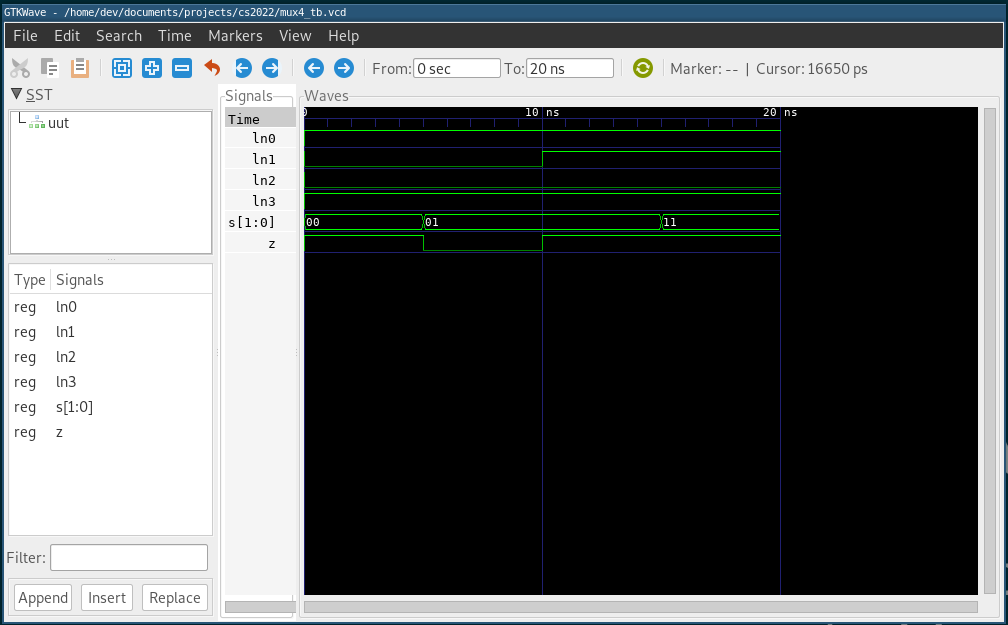
\includegraphics[width=\textwidth]{mux4_tb}
	\caption{\mi{c}{mux4} testbench results}
	\label{fig:mux4}
\end{figure}

Figure~\ref{fig:mux4} shows the simulation results of a simple 4-to-1 mux.
\begin{itemize}
	\item When \mi{c}{s = 00}, \mi{c}{z = 1} since \mi{c}{ln0 = 1}
	\item Changing \mi{c}{s = 01} results in \mi{c}{z = 0} as \mi{c}{ln1 = 0}
	\item Later \mi{c}{ln1 = 1}, at which point \mi{c}{z = 1}
	\item Finally, with \mi{c}{s = 11}, \mi{c}{z} remains the same since \mi{c}{ln3 = 1}
\end{itemize}

\emph{Note: testbenches for \mi{c}{mux2} and \mi{c}{mux3} were not included since they are simply 
reduced versions of \mi{c}{mux4}.}

\newpage
\subsection{\mi{c}{full_adder}}
\begin{figure}[h!]
	\centering
	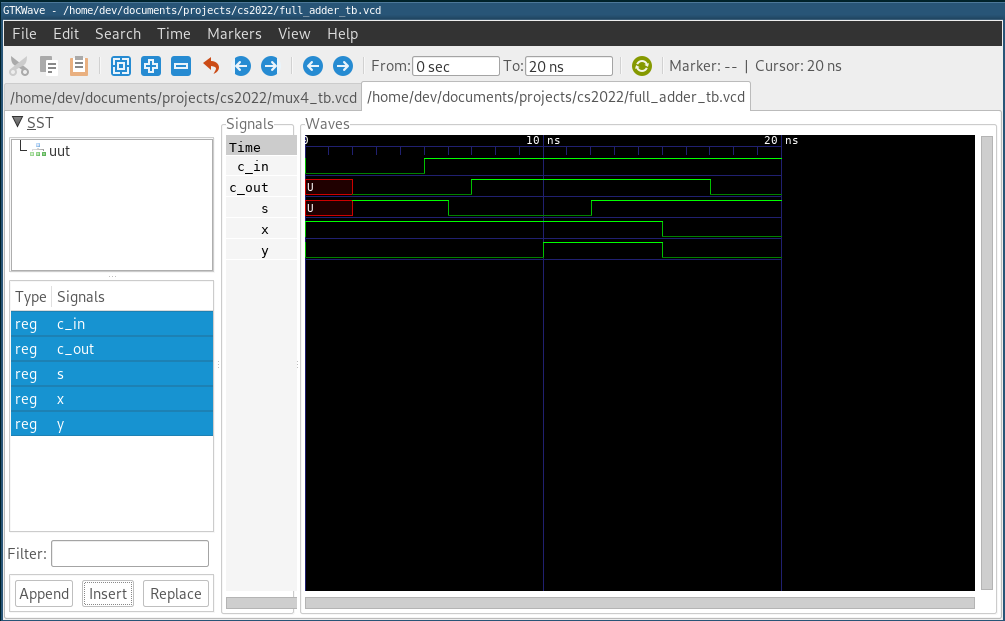
\includegraphics[width=\textwidth]{full_adder_tb}
	\caption{\mi{c}{full_adder} testbench results}
	\label{fig:fulladder}
\end{figure}

Figure~\ref{fig:fulladder} shows the simulation results of a gate-level full adder.
\begin{itemize}
	\item Initially, \mi{c}{x = 1}, \mi{c}{y = 0} and there is no carry in - as such the sum is 1 and there is no carry out
	\item Adding a carry in results in the sum being 0 and a carry out
	\item Setting \mi{c}{y = 1} results in both sum and carry out being active
	\item With only a carry in, the sum is 1 and there is no carry out
\end{itemize}

\newpage
\subsection{\mi{c}{arith_b_fn}}
\begin{figure}[h!]
	\centering
	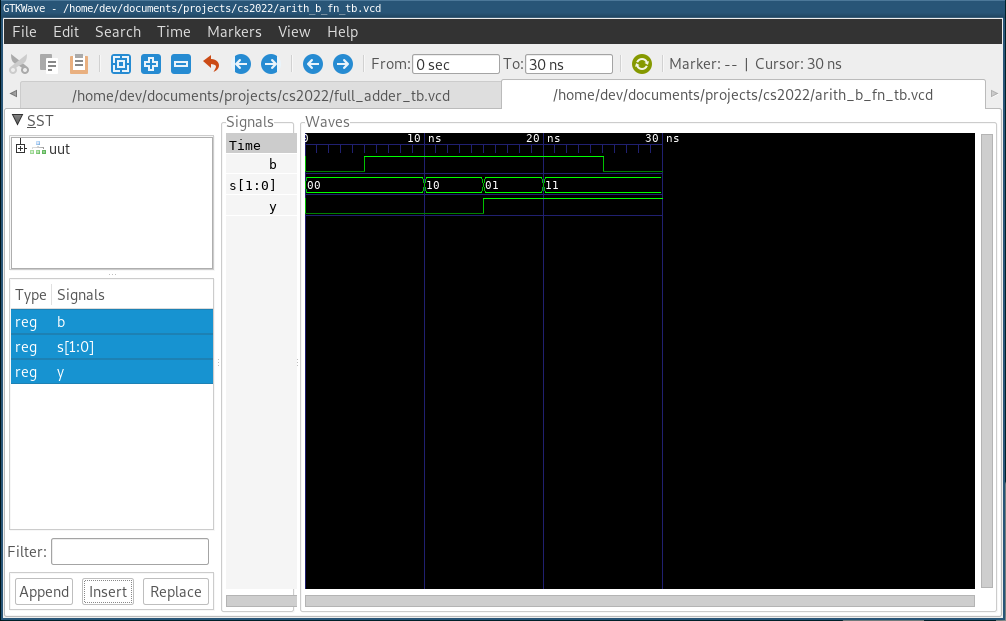
\includegraphics[width=\textwidth]{arith_b_fn_tb}
	\caption{\mi{c}{arith_b_fn} testbench results}
	\label{fig:arithb}
\end{figure}

Figure~\ref{fig:arithb} shows the simulation results of the b logic function (implemented with a mux).
\begin{itemize}
	\item With \mi{c}{s = 00}, the output is 0 (all zeroes)
	\item \mi{c}{s = 10}, the output is 0 (\mi{c}{!b})
	\item \mi{c}{s = 01}, the output is 1 (\mi{c}{b})
	\item \mi{c}{s = 11}, the output is 1 (all ones)
\end{itemize}
\emph{Note: The values of \mi{c}{s} for \mi{c}{!b} and \mi{c}{b} have been swapped in order to fix match the required micro op format}

\newpage
\subsection{\mi{c}{arithmetic_slice}}
\begin{figure}[h!]
	\centering
	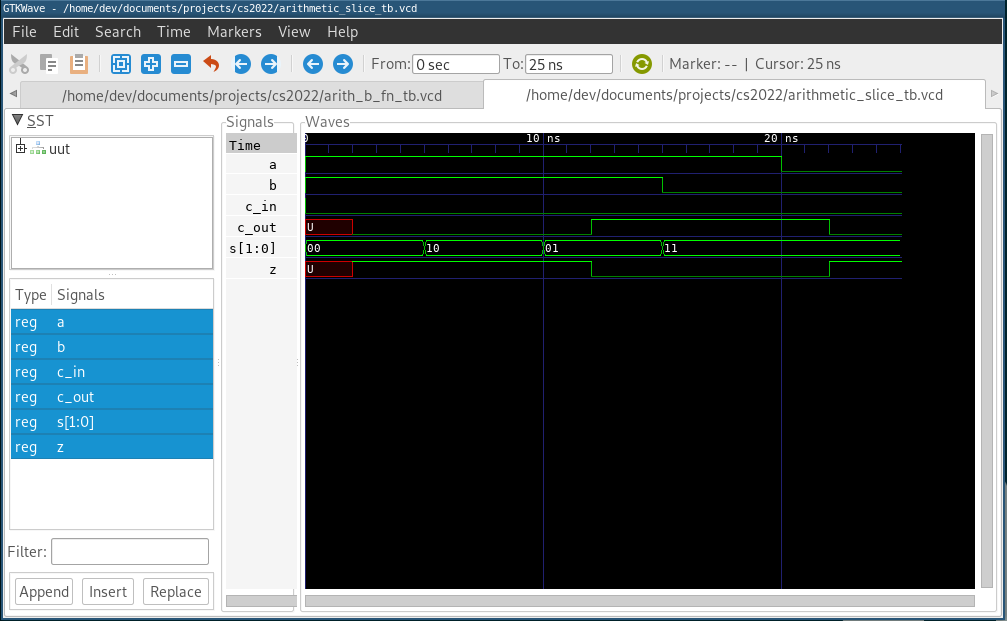
\includegraphics[width=\textwidth]{arithmetic_slice_tb}
	\caption{\mi{c}{arithmetic_slice} testbench results}
	\label{fig:arithslice}
\end{figure}

Figure~\ref{fig:arithslice} shows the simulation results of the arithmetic slice, which is a 
full adder with the second operand coming from the b logic function.

\newpage
\subsection{\mi{c}{logic_slice}}
\begin{figure}[h!]
	\centering
	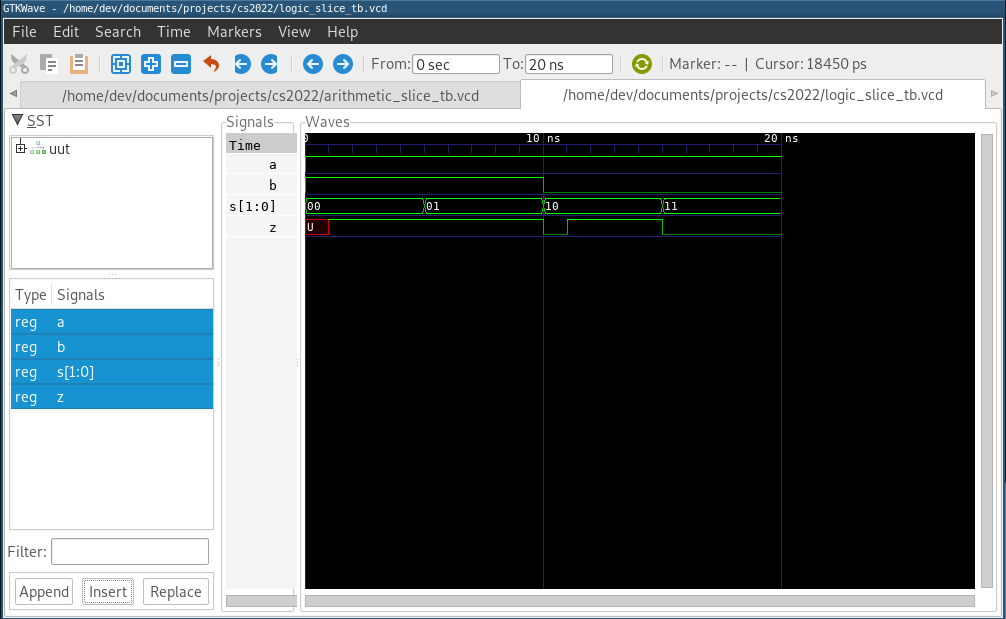
\includegraphics[width=\textwidth]{logic_slice_tb}
	\caption{\mi{c}{logic_slice} testbench results}
	\label{fig:logicslice}
\end{figure}

Figure~\ref{fig:logicslice} shows the simulation results of the logic slice (implemented with a mux and simple gates).
\begin{itemize}
	\item Initially, \mi{c}{a = b = 1} and \mi{c}{s = 00} - the output is 1 (\mi{c}{a & b})
	\item Changing \mi{c}{s = 01} gives 1 (\mi{c}{a | b})
	\item With \mi{c}{s = 10} and \mi{c}{b = 0}, the output is 1 after gate propagation (\mi{c}{a ^ b})
	\item \mi{c}{s = 11} gives 0 (\mi{c}{!a})
\end{itemize}

\newpage
\subsection{\mi{c}{alu_slice}}
\begin{figure}[h!]
	\centering
	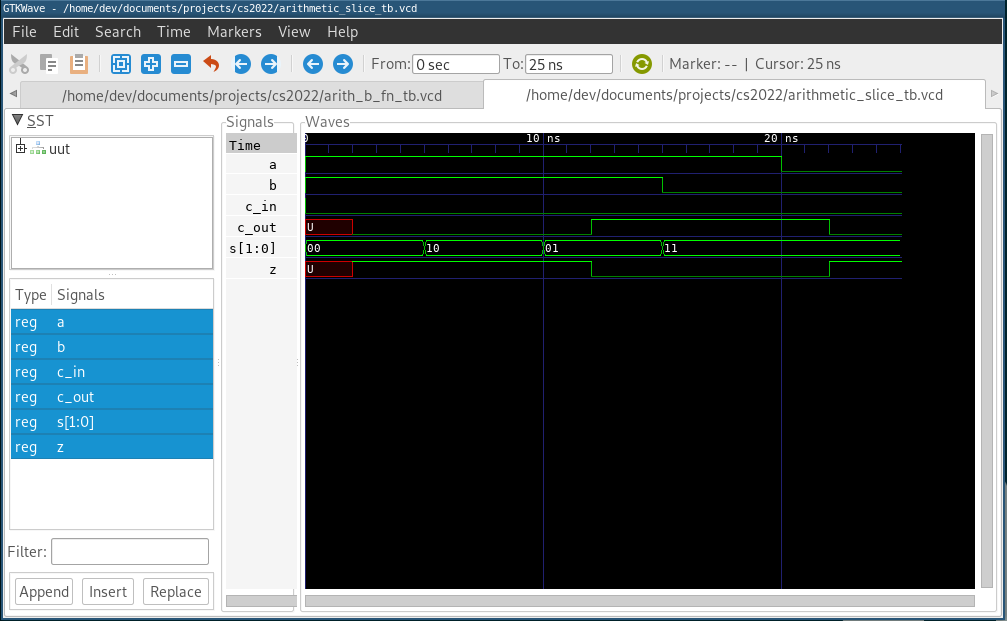
\includegraphics[width=\textwidth]{arithmetic_slice_tb}
	\caption{\mi{c}{alu_slice} testbench results}
	\label{fig:aluslice}
\end{figure}

Figure~\ref{fig:aluslice} shows the simulation results of the ALU slice, which is a 
combination of an arithmetic slice and a logic slice, where the operation type (arithmetic or 
logical) is selected by a mux (which is controlled by an additional \mi{c}{s} bit).

\newpage
\subsection{\mi{c}{alu}}
\begin{figure}[h!]
	\centering
	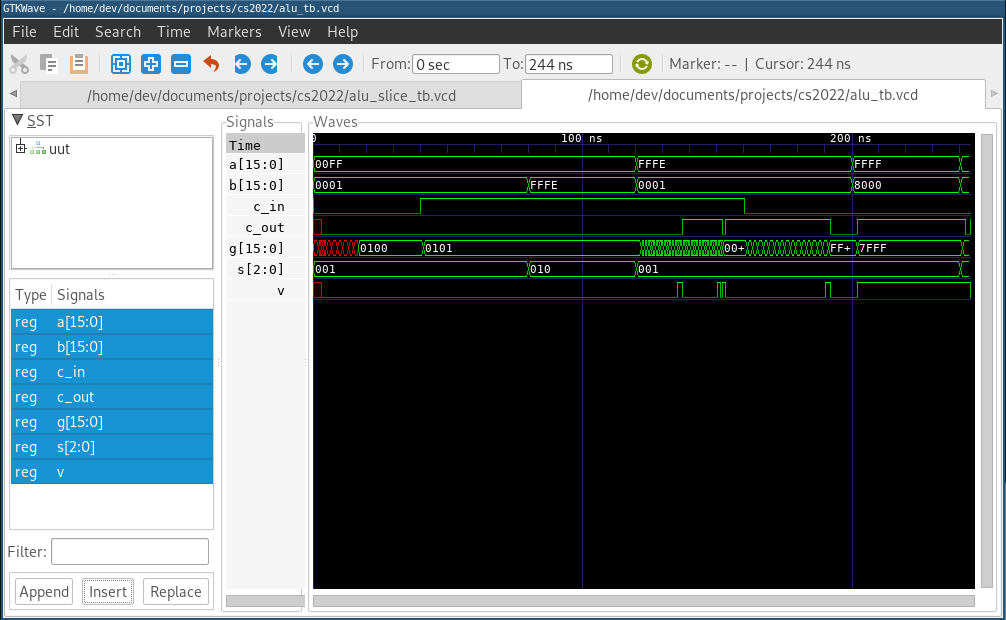
\includegraphics[width=\textwidth]{alu_tb}
	\caption{\mi{c}{alu} testbench results}
	\label{fig:alu}
\end{figure}

Figure~\ref{fig:alu} shows the simulation results of the complete ALU, which is formed
using VHDL \mi{vhdl}{generate} blocks to instantiate 16 ALU slices and connect them together.

The functionality is identical to the ALU slice, except for the size of the operands (and 
associated ripple delay). There is also a signed overflow flag, which is calculated by \mi{c}{xor}'ing 
the carry in and carry out of the most significant bit's ALU slice. It can be seen functioning when
adding \mi{c}{0xffff} (-1) and \mi{c}{0x8000} (-32768), giving an erroneous result of 
\mi{c}{0x7fff} (32767).

\newpage
\subsection{\mi{c}{shifter}}
\begin{figure}[h!]
	\centering
	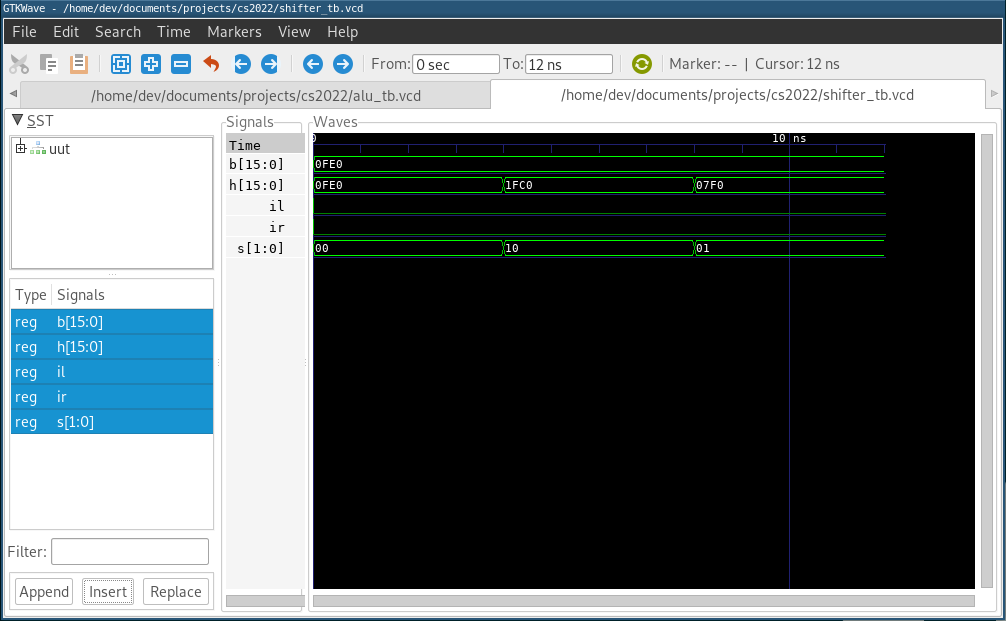
\includegraphics[width=\textwidth]{shifter_tb}
	\caption{\mi{c}{shifter} testbench results}
	\label{fig:shifter}
\end{figure}

Figure~\ref{fig:shifter} shows the simulation results of a 16-bit shifter, which is formed
using VHDL \mi{vhdl}{generate} blocks to instantiate 3-to-1 muxes which perform the shifting 
functionality.
\begin{itemize}
	\item When \mi{c}{s = 00}, the output is the same as the input
	\item With \mi{c}{s = 10}, \mi{c}{0x0fe0} becomes \mi{c}{0x1fc0} (shifted left)
	\item \mi{c}{s = 01} gives \mi{c}{0x1fc0} (shifted right)
\end{itemize}

\newpage
\subsection{\mi{c}{function_unit}}
\begin{figure}[h!]
	\centering
	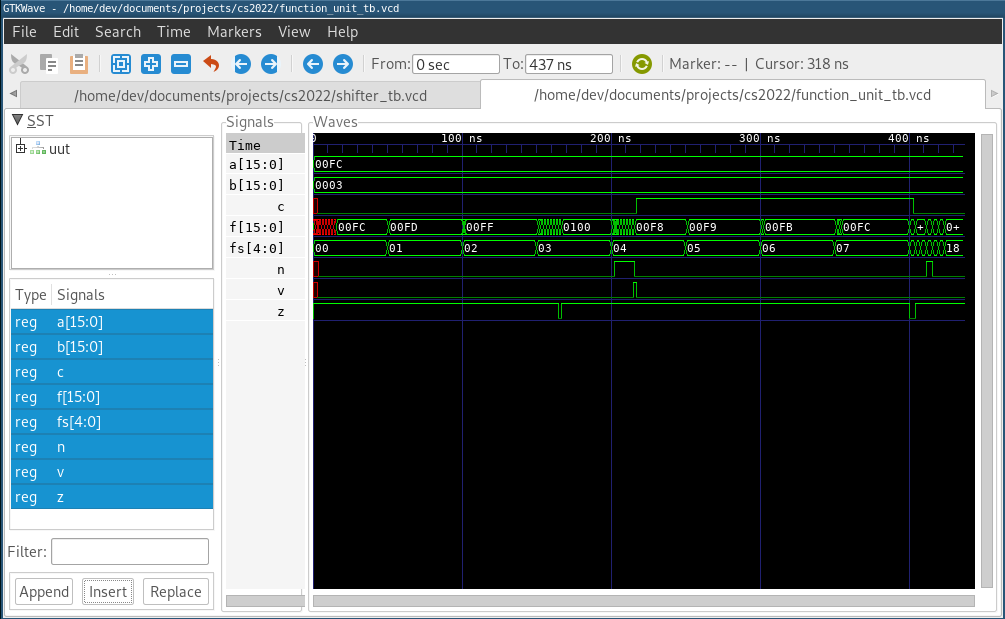
\includegraphics[width=\textwidth]{function_unit_tb}
	\caption{\mi{c}{function_unit} testbench results}
	\label{fig:fnu}
\end{figure}
Figure~\ref{fig:fnu} shows the simulation results of the complete function unit, which consists of
an ALU, a shifter and a 16-bit mux to select the output.

In addition to passing through the overflow flag and carry out from the ALU, a negative flag 
(active if the most significant bit of the output is set) and zero flag (if the output is 0).

\mi{c}{fs} determines the micro op performed by the function unit on the inputs:
\begin{itemize}
	\item \mi{vhdl}{fs(0)} is the carry in for the ALU
	\item \mi{vhdl}{fs(4)} determines if the operation should be arithmetic / logical or a shift
	\item \mi{vhdl}{fs(3 downto 1)} provides \mi{c}{s} for the ALU
	\item \mi{vhdl}{fs(3 downto 2)} provides \mi{c}{s} for the shifter
\end{itemize}

\newpage
\subsection{\mi{c}{register_file}}
\begin{figure}[h!]
	\centering
	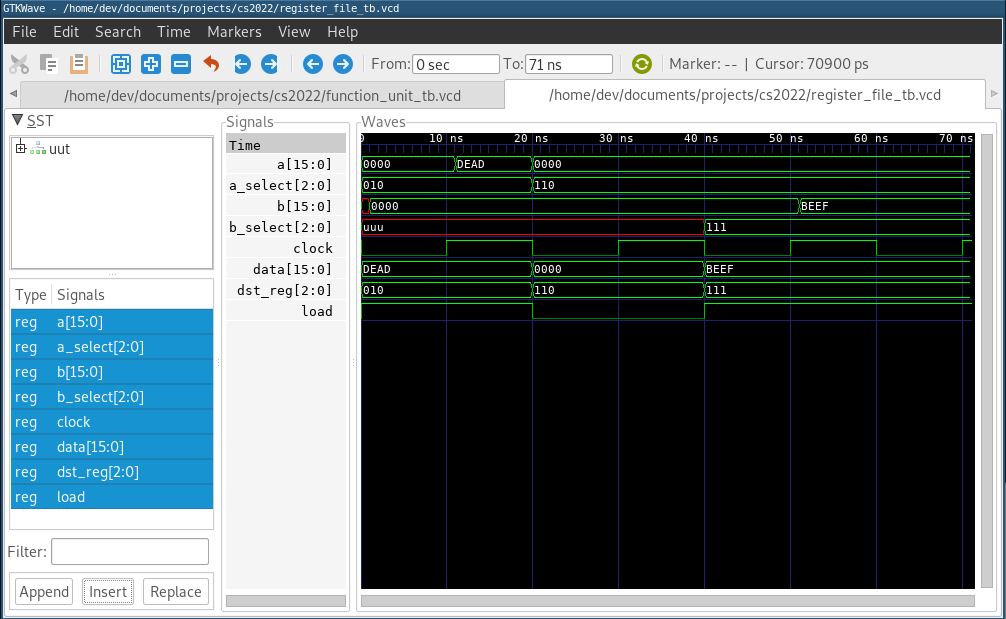
\includegraphics[width=\textwidth]{register_file_tb}
	\caption{\mi{c}{register_file} testbench results}
	\label{fig:regs}
\end{figure}

Figure~\ref{fig:regs} shows the simulation results of the updated register file.
\begin{itemize}
	\item Firstly, \mi{c}{0xdead} is loaded into \mi{c}{r2} by setting \mi{c}{data = 0xdead}, \mi{c}{dst_reg = 2} and \mi{c}{load = 1} - \mi{c}{a_select} is also set to 2 and the loaded result can be seen in the \mi{c}{a} output after a clock pulse
	\item 0 is then loaded into \mi{c}{r6} and seen on the a output
	\item Finally, \mi{c}{0xbeef} is loaded into \mi{c}{r7} and seen on the b output
\end{itemize}

\newpage
\subsection{\mi{c}{datapath}}
\begin{figure}[h!]
	\centering
	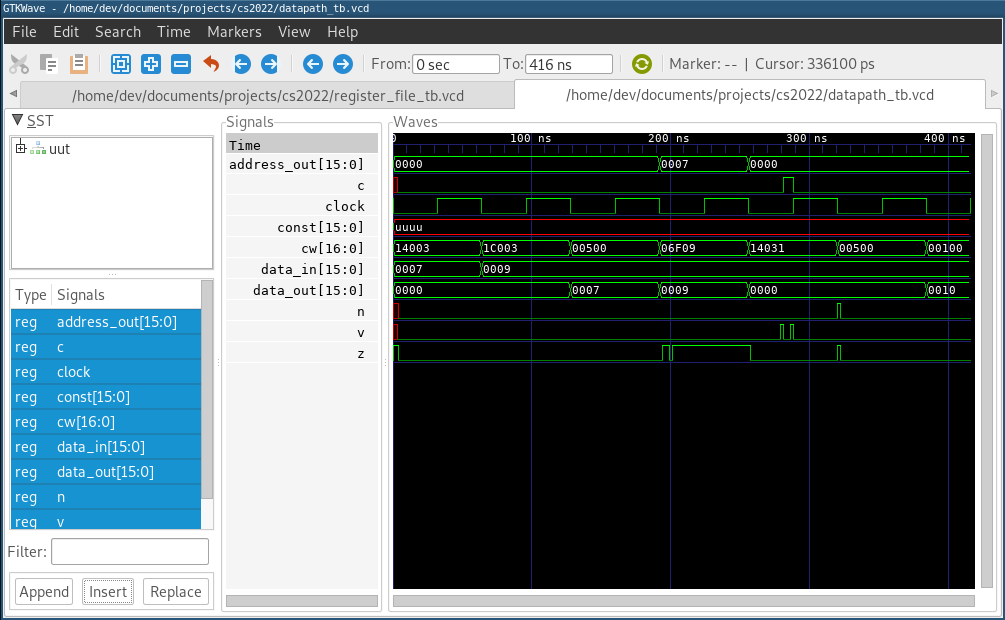
\includegraphics[width=\textwidth]{datapath_tb}
	\caption{\mi{c}{datapath} testbench results}
	\label{fig:datapath}
\end{figure}

Figure~\ref{fig:datapath} shows the simulation results of the complete 16-bit datapath.
It consists of the updated register file, the function unit, a mux to select the source of 
data loaded into registers (function unit or \mi{c}{data_in}) and a mux to select the source 
of the b input to the function unit (register file b output or constant).

All control is performed by a 17-bit control word:
\begin{itemize}
	\item Register file \mi{vhdl}{dst_reg <= cw(16 downto 14)}
	\item Register file \mi{vhdl}{a_select <= cw(13 downto 11)}
	\item Register file \mi{vhdl}{b_select <= cw(10 downto 8)}
	\item \mi{vhdl}{cw(7)} is the function unit b operand source select
	\item Function unit control \mi{vhdl}{fs <= cw(6 downto 2)}
	\item \mi{vhdl}{cw(1)} is the register file \mi{c}{data_in} source select
	\item Register file \mi{vhdl}{load <= cw(0)}
\end{itemize}

The micro ops performed by the testbench are (approximately):
\begin{itemize}
	\item \mi{c}{r5 <- 7}
	\item \mi{c}{r7 <- 9}
	\item \mi{c}{data_out <- r5}
	\item \mi{c}{add r1, r5, r7}
	\item \mi{c}{xor r5, r0, r0}
	\item \mi{c}{data_out <- r5}
	\item \mi{c}{data_out <- r1}
\end{itemize}

\end{document}
# vim: nofoldenable
